%% Preamble %%
%% A minimal LaTeX preamble
%% Some packates are needed to implement
%% Asciidoc features

\documentclass[12pt]{article}
\usepackage[brazilian]{babel}
\usepackage[left=3.00cm, right=2.00cm, top=3.00cm, bottom=2.00cm]{geometry}                % See geometry.pdf to learn the layout options. There are lots.
%\geometry{letterpaper}               % ... or a4paper or a5paper or ...
%\geometry{landscape}                % Activate for for rotated page geometry
%\usepackage[parfill]{parskip}       % Activate to begin paragraphs with an empty line rather than an indent

\usepackage{tcolorbox}
\usepackage{lipsum}

\usepackage{epstopdf}
\usepackage{color}
% \usepackage[usenames, dvipsnames]{color}
% \usepackage{alltt}


\usepackage{amssymb}
% \usepackage{amsmath}
\usepackage{amsthm}
\usepackage{cancel}
\usepackage[version=3]{mhchem}


% Needed to properly typeset
% standard unicode characters:
%
\RequirePackage{fix-cm}
\usepackage{fontspec}
\usepackage[Latin,Greek]{ucharclasses}
%
% NOTE: you must also use xelatex
% as the typesetting engine


% \usepackage{fontspec}
% \usepackage{polyglossia}
% \setmainlanguage{en}

\usepackage{hyperref}
\hypersetup{
    colorlinks=true,
    linkcolor=blue,
    filecolor=magenta,
    urlcolor=blue,
}

\usepackage{graphicx}
\usepackage{wrapfig}
\graphicspath{ {images/} }
\DeclareGraphicsExtensions{.png, .jpg, jpeg, .pdf}

%% \DeclareGraphicsRule{.tif}{png}{.png}{`convert #1 `dirname #1`/`basename #1 .tif`.png}
%% Asciidoc TeX Macros %%


% \pagecolor{black}
%%%%%%%%%%%%


% Needed for Asciidoc

\newcommand{\admonition}[2]{\textbf{#1}: {#2}}
\newcommand{\rolered}[1]{ \textcolor{red}{#1} }
\newcommand{\roleblue}[1]{ \textcolor{blue}{#1} }

\newtheorem{theorem}{Theorem}
\newtheorem{proposition}{Proposition}
\newtheorem{corollary}{Corollary}
\newtheorem{lemma}{Lemma}
\newtheorem{definition}{Definition}
\newtheorem{conjecture}{Conjecture}
\newtheorem{problem}{Problem}
\newtheorem{exercise}{Exercise}
\newtheorem{example}{Example}
\newtheorem{note}{Note}
\newtheorem{joke}{Joke}
\newtheorem{objection}{Objection}





%%%%%%%%%%%%%%%%%%%%%%%%%%%%%%%%%%%%%%%%%%%%%%%%%%%%%%%

%  Extended quote environment with author

\renewenvironment{quotation}
{   \leftskip 4em \begin{em} }
{\end{em}\par }

\def\signed#1{{\leavevmode\unskip\nobreak\hfil\penalty50\hskip2em
  \hbox{}\nobreak\hfil\raise-3pt\hbox{(#1)}%
  \parfillskip=0pt \finalhyphendemerits=0 \endgraf}}


\newsavebox\mybox

\newenvironment{aquote}[1]
  {\savebox\mybox{#1}\begin{quotation}}
  {\signed{\usebox\mybox}\end{quotation}}

\newenvironment{tquote}[1]
  {  {\bf #1} \begin{quotation} \\ }
  { \end{quotation} }

%% BOXES: http://tex.stackexchange.com/questions/83930/what-are-the-different-kinds-of-boxes-in-latex
%% ENVIRONMENTS: https://www.sharelatex.com/learn/Environments

\newenvironment{asciidocbox}
  {\leftskip6em\rightskip6em\par}
  {\par}

\newenvironment{titledasciidocbox}[1]
  {\leftskip6em\rightskip6em\par{\bf #1}\vskip-0.6em\par}
  {\par}



%%%%%%%%%%%%%%%%%%%%%%%%%%%%%%%%%%%%%%%%%%%%%%%%%%%%%%%%

%% http://texblog.org/tag/rightskip/


\newenvironment{preamble}
  {}
  {}

%% http://tex.stackexchange.com/questions/99809/box-or-sidebar-for-additional-text
%%
\newenvironment{sidebar}[1][r]
  {\wrapfigure{#1}{0.5\textwidth}\tcolorbox}
  {\endtcolorbox\endwrapfigure}


%%%%%%%%%%

\newenvironment{comment*}
  {\leftskip6em\rightskip6em\par}
  {\par}

  \newenvironment{remark*}
  {\leftskip6em\rightskip6em\par}
  {\par}


%% Dummy environment for testing:

\newenvironment{foo}
  {\bf Foo.\ }
  {}


\newenvironment{foo*}
  {\bf Foo.\ }
  {}


\newenvironment{click}
  {\bf Click.\ }
  {}

\newenvironment{click*}
  {\bf Click.\ }
  {}

\newenvironment{resposta}
{\bf Resposta:\\ }
{}

\newenvironment{resposta*}
{\bf Resposta:\\ }
{}


\newenvironment{remark}
  {\bf Remark.\ }
  {}

\newenvironment{capsule}
  {\leftskip10em\par}
  {\par}

%%%%%%%%%%%%%%%%%%%%%%%%%%%%%%%%%%%%%%%%%%%%%%%%%%%%%

%% Style

\parindent0pt
\parskip8pt
%% User Macros %%
%% Front Matter %%

\title{Termodinâmica}
\author{Jefferson Rodrigues de Oliveira}
\date{}


%% Begin Document %%

\begin{document}
\maketitle
\tableofcontents
\hypertarget{x-objetivos}{\section{Objetivos}}
Caro aluno, logo abaixo apresentarei \textbf{os principais objetivos que você deve alcançar} ao estudar este conteúdo:


\begin{itemize}

\item \textbf{Compreender} processos em que o fornecimento de calor a um sistema, ou corpo, pode produzir aumento de seu volume, resultando na realização de trabalho.

\item \textbf{Compreender} o primeiro princípio da termodinâmica: a quantidade de calor fornecida a um sistema é igual ao trabalho que ele realiza mais a variação de sua energia interna.

\item \textbf{Compreender} que o Primeiro Princípio da Termodinâmica expressa quantitativamente a Lei de Conservação da Energia.

\item \textbf{Saber aplicar} o Primeiro Princípio da Termodinâmica para resolver problemas envolvendo calor, trabalho e energia interna de um sistema.

\item \textbf{Compreender} que o funcionamento de máquinas térmicas requer sempre troca de calor entre duas fontes, uma quente e outra fria.

\item \textbf{Compreender} que, numa máquina térmica, só uma parte do calor fornecido é transformado em trabalho.

\end{itemize}


\hypertarget{x-introdução}{\section{Introdução}}
Primeiramente, temos que compreender o \textbf{contexto histórico} relacionado com o tema em estudo. No \textbf{século XVIII} surgiram as primeiras máquinas a vapor, nelas o valor aquecido em um cilindro, empurra um pistão em que produz o movimento desejado. Desta forma, temos a transformação de calor em trabalho. Essas máquinas desempenharam um papel bastante importante durante a \textbf{Revolução Industrial}.


\begin{figure}[h]{}
\centering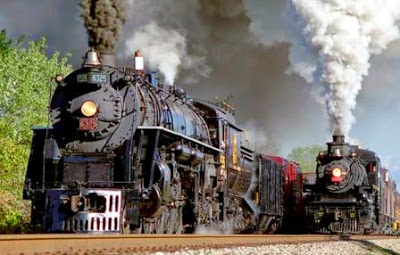
\includegraphics[width=2.5truein]{img1.jpg}
\caption{Transformação de calor em trabalho. Fonte: osfundamentosdafisica}
\centering
\end{figure}

Durante o século XIX, o \textbf{calor} foi reconhecido com uma \textbf{forma de energia} e que foi estabelecido o \textbf{Princípio da Conservação da Energia}. Nessa época, passou-se a usar o termo \textbf{Termodinâmica} para designar o estudo das transformações entre energia mecânica (\textbf{trabalho}) em energia térmica (\textbf{calor}).


As \textbf{Leis da Termodinâmica} que iremos estudar, valem para quaisquer sistemas: sólidos, líquidos ou gasosos; no entanto, iremos aplicá-las apenas nos casos \textbf{mais simples}, ou seja, no caso em que o sistema estudado é um \textbf{gás ideal}. Portanto, antes de estudarmos essas leis, vamos primeiramente comentar alguns fatos relacionados ao comportamento dos gases ideais.


\hypertarget{x-energia-interna,-trabalho-e-calor}{\section{Energia interna, trabalho e calor}}
No estudo da \textbf{Termodinâmica dos Gases Ideais}, são parâmetros básicos as grandezas físicas: \textbf{energia interna ($U$)}, \textbf{trabalho ($\tau$)} e a \textbf{quantidade de calor ($Q$)}.


Veremos, logo a seguir, como funciona cada uma destes três parâmetros.


\hypertarget{x-energia-interna}{\subsection{Energia interna}}
\textbf{A energia interna de um sistema é o somatório de vários tipos de energia existentes em suas partículas}. Como vimos, no caso de uma gás perfeito (\textbf{monoatômico}) a energia interna se resume na \textbf{energia de translação de suas partículas} e, seu cálculo é o seguinte:


\begin{equation}\label{eq:energiainterna}
    U=\dfrac{3}{2}nRT
\end{equation}


Ou seja, a anergia interna depende apenas da temperatura (\textbf{$T$}) do sistema e varia de forma \textbf{linear} (pois é uma função de 1° grau).


Para uma transformação termodinâmica de uma gás monoatômico de $A\Rightarrow B$, temos que:


\begin{equation*}
    \Delta U = \dfrac{3}{2}nR\Delta T
\end{equation*}


Onde $\Delta T = T_{B}-T_{A}$.


Portanto:


\begin{itemize}

\item \textbf{$T$} aumenta $\Rightarrow$ \textbf{$\Delta U > 0$}: a energia interna do gás aumenta.

\item \textbf{$T$} diminui $\Rightarrow$ \textbf{$\Delta U < 0$}: a energia interna do gás diminui.

\item \textbf{$T$} constante $\Rightarrow$ \textbf{$\Delta U = 0$}: a energia interna do gás não é alterada.

\end{itemize}


\textbf{Observação}: se o gás não for monoatômico, outras formas de energia devem ser levadas em conta como, por exemplo, a energia cinética de rotação das moléculas. Nestas condições, teremos:


\begin{equation*}
    U > \dfrac{3}{2}nRT
\end{equation*}


Por fim, se relacionarmos a equação da energia interna com a Lei de Clapeyron ($PV = nRT$), encontraremos:


\begin{equation}
    U = \dfrac{3}{2}pV\\
\end{equation}


\hypertarget{x-trabalho}{\subsection{Trabalho}}
De acordo como o que já foi estudado em \textbf{Mecânica}, sabemos que todo \textbf{trabalho} é realizado por uma \textbf{força}. Vamos então considerar a \textbf{expansão} de um \textbf{gás perfeito} submetido a uma pressão constante (\textbf{transformação isobárica}).


\begin{figure}[h]{}
\centering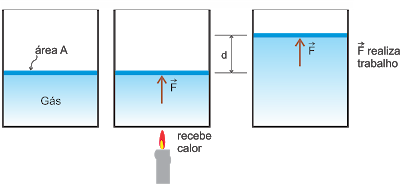
\includegraphics[width=2.5truein]{img2.png}
\caption{Trabalho de um gás. Fonte: osfundamentosdafisica}
\centering
\end{figure}

\begin{align*}
    \tau &= Fd \\
    \tau &= pAd
\end{align*}


Mas, $Ad=\Delta V$ (variação de volume). Portanto:


\begin{equation}\label{eq:trabalho}
    \tau = p\Delta V
\end{equation}


Analisando o diagrama $p\times V$:


\begin{figure}[h]{}
\centering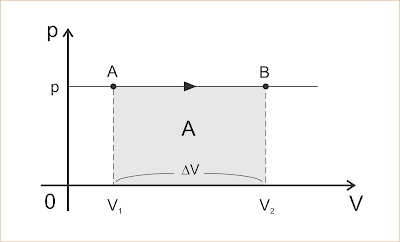
\includegraphics[width=2.5truein]{img3.png}
\caption{Diagrama I. Fonte: osfundamentosdafisica}
\centering
\end{figure}

A área (\textbf{$A$}) do retângulo do diagrama acima é numericamente igual ao trabalho (\textbf{$\tau$}). De fato podemos perceber isto:


\begin{align*}
    \text{Área} &= \text{base} \times \text{altura} \\
    A &= bh \\
    A &= p\Delta V
\end{align*}


Sendo assim, podemos concluir que, em uma \textbf{transformação isobárica}, de fato, \textbf{o trabalho realizado é numericamente igual a área abaixo da curva}.


Isso não é um fato exclusivo para este tipo de transformação. É possível fazer uma generalização para quaisquer tipo de transformação utilizando ferramentas de matemática superior, mas acredite, \textbf{vale para qualquer tipo de transformação}.


Para analisar o trabalho de uma transformação, podemos adotar o seguinte:


\begin{itemize}

\item \textbf{$V$} aumenta $\Rightarrow$ \textbf{$\tau > 0$}: o gás \textbf{realiza} trabalho.

\item \textbf{$V$} diminui $\Rightarrow$ \textbf{$\tau < 0$}: o gás \textbf{recebe} trabalho.

\item \textbf{$V$} constante $\Rightarrow$ \textbf{$\tau = 0$}: o gás \textbf{não realiza} trabalho.

\end{itemize}


\textbf{Exercício Resolvido 1}


Um gás sofre uma transformação \textbf{$A\Rightarrow B$} conforme indica o diagrama \textbf{$p\times V$}. Calcule o trabalho que o gás troca com o meio exterior.


\begin{figure}[h]{}
\centering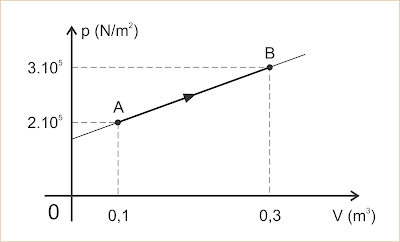
\includegraphics[width=2.5truein]{img4.1.png}
\caption{Diagrama. Fonte: osfundamentosdafisica}
\centering
\end{figure}

\begin{resposta*}
{\it O trabalho pode ser calculado como numericamente igual a área abaixo da curva (neste caso, um trapézio).

\begin{align*}
    A &= \dfrac{(B+b)h}{2}\\
    A &= \dfrac{(3\times 10^{5}+2\times 10^{5})(0,3-0,1)}{2}\\
    A &= \dfrac{(5\times 10^{5})(0,2)}{2}\\
    A &= 5\times 10^{4}\;J
\end{align*}

Sendo assim, $\boxed{\tau = 5\times 10^{4}\;J}$

Perceba que o sinal \textbf{deve ser positivo}, pois o gás \textbf{realiza trabalho} (o volume do gás aumenta). $\blacksquare$}
\end{resposta*}

Caso o gás percorra um ciclo (\textbf{transformação cíclica}), isto é, o estado final coincide com o inicial, o trabalho trocado com o sistema é \textbf{numericamente igual a área do ciclo}.


\begin{equation*}
    \tau \stackrel{N}{=} A
\end{equation*}


\begin{figure}[h]{}
\centering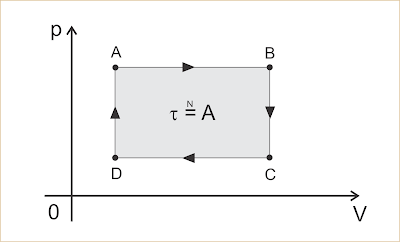
\includegraphics[width=2.5truein]{img5.png}
\caption{Diagrama. Fonte: osfundamentosdafisica}
\centering
\end{figure}

Podemos perceber que na transformação \textbf{$A\Rightarrow B$} o gás \textbf{realiza} trabalho e em \textbf{$C\Rightarrow D$}, \textbf{recebe}. O trabalho realizado é, em módulo, maior do que o recebido. Logo, \textbf{quando o ciclo é percorrido no sentido horário o gás realiza trabalho sobre o meio exterior}. Analogamente, \textbf{quando o ciclo é percorrido no sentido anti-horário o gás recebe trabalho do meio exterior}.


\begin{figure}[h]{}
\centering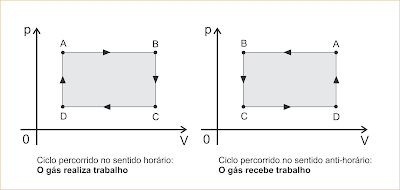
\includegraphics[width=2.5truein]{img6.png}
\caption{Diagrama. Fonte: osfundamentosdafisica}
\centering
\end{figure}

\textbf{Exercício Resolvido 2}


Um gás sofre ume transformação cíclica $ABCDA$, conforme indicado no diagrama $p\times V$.


\begin{figure}[h]{}
\centering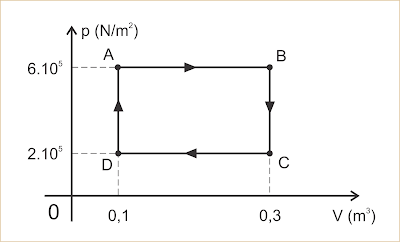
\includegraphics[width=2.5truein]{img7.png}
\caption{Diagrama. Fonte: osfundamentosdafisica}
\centering
\end{figure}

a) Sendo $T_{A} = 300\;K$ a temperatura no estado representado pelo ponto $A$, determine as temperaturas em $B$, $C$ e $D$. \\
b) Calcule o trabalho que o gás troca com o meio exterior ao percorrer o ciclo. Neste ciclo o gás realiza ou recebe trabalho do meio exterior?


\begin{resposta*}
{\it a) $A\Rightarrow B$: \textbf{transformação isobárica}:

\begin{align*}
    \frac{V_{A}}{T_{A}} &= \dfrac{V_{B}}{T_{B}} \\
    T_{B} &= T_{A}\left(\dfrac{V_{B}}{V_{A}}\right) \\
    T_{B} &= 300\left(\dfrac{0,3}{0,1}\right) \\
    T_{B} &= 900
\end{align*}

Ou seja, $\boxed{T_{B} = 900\;K}$ \\

$B\Rightarrow C$: \textbf{transformação isocórica}:

\begin{align*}
    \frac{P_{B}}{T_{B}} &= \dfrac{P_{C}}{T_{C}} \\
    T_{C} &= T_{B}\left(\dfrac{P_{C}}{P_{B}}\right) \\
    T_{C} &= 900\left(\dfrac{2\times 10^{5}}{6\times 10^{5}}\right) \\
    T_{C} &= 300
\end{align*}

Ou seja, $\boxed{T_{C} = 300\;K}$ \\

$C\Rightarrow D$: \textbf{transformação isobárica}:
\begin{align*}
    \frac{V_{C}}{T_{C}} &= \dfrac{V_{D}}{T_{D}} \\
    T_{D} &= T_{C}\left(\dfrac{V_{D}}{V_{C}}\right) \\
    T_{D} &= 300\left(\dfrac{0,1}{0,3}\right) \\
    T_{D} &= 100
\end{align*}

Ou seja, $\boxed{T_{D} = 100\;K}$ \\

b) Aqui podemos utilizar a relação que o trabalho é numericamente igual a área do ciclo.

\begin{align*}
    A &= bh \\
    A &= (0,3-0,1)(6\times 10^{5}-2\times 10^{5}) \\
    A &= (0,2)(4\times 10^{5}) \\
    A &= 8\times 10^{4}
\end{align*}

Ou seja, $\boxed{\tau = 8\times 10^{4}\;J}$

Perceba que o sinal do trabalho deve ser \textbf{positivo}, pois o ciclo é percorrido no \textbf{sentido horário} (o gás \textbf{realiza} trabalho). $\blacksquare$}
\end{resposta*}

\hypertarget{x-calor}{\subsection{Calor}}
Já estudamos que o calor é a energia térmica transitando de um sistema para outro. Assim, um dos sistemas cede essa energia e o outro, a recebe. Por convenção, \textbf{o calor recebido é positivo e o calor cedido, negativo}.


\hypertarget{x-lei-zero-da-termodinâmica}{\section{Lei Zero da Termodinâmica}}
Como também já estudamos, A \textbf{Lei Zero da Termodinâmica trabalha o conceito de equilíbrio térmico}. Essa lei diz que dois sistemas físicos estão em equilíbrio se, ao serem colocados em contato térmico, não há fluxo de calor entre eles. Sendo assim, se dois sistemas físicos, \textbf{A} e \textbf{B}, estão individualmente em equilíbrio térmico com um terceiro sistema \textbf{C}, então ambos estarão em equilíbrio térmico entre si (se $T_{a}=T_{c}$ e $T_{b}=T_{c}$, então $T_{a}=T_{b}$).


\hypertarget{x-primeira-lei-da-termodinâmica}{\section{Primeira Lei da Termodinâmica}}
A \textbf{1ª Lei da Termodinâmica} é a aplicação do \textbf{Princípio  da Conservação  da Energia}. Com a aplicação desta Lei, podemos, por meio de uma "contagem" energética, saber o que ocorrer um sistema gasoso ao sobre uma transformação termodinâmica.


Imagine que um gás receba uma quantidade de calor igual $Q = 100\;J$. Vamos supor que o gás se expanda e realize um trabalho $\tau = 80\;J$. Os $20\;J$ restantes ficam armazenados no gás, aumentando sua energia interna ($\Delta U=20\;J$). As três formas de energia, $Q$,  $\tau$  e $\Delta U$ relacionam-se, constituindo a primeira lei da Termodinâmica:


\textbf{Para todo sistema termodinâmico existe uma função característica denominada energia interna. A variação dessa energia interna ($\Delta U$) entre dois estados quaisquer pode ser determinada  pela diferença entre a quantidade de calor ($Q$) e o trabalho ($\tau$) trocados com o meio externo.}


Matematicamente,


\begin{equation}
    \Delta U=Q-\tau
\end{equation}


\hypertarget{x-transformação-isotérmica}{\subsection{Transformação Isotérmica}}
Nas \textbf{transformações isotérmicas}, a temperatura do sistema se matem constante e, consequentemente, \textbf{a variação de energia interna é nula ($\Delta u=0$)}.


\begin{figure}[h]{}
\centering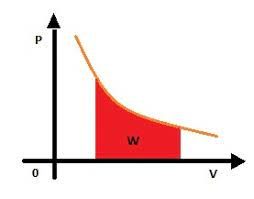
\includegraphics[width=2.5truein]{img8.jpg}
\caption{Transformação isotérmica. Fonte: wikimedia}
\centering
\end{figure}

Aplicando a 1º Lei da Termodinâmica neste tipo de transformação, temos:


\begin{align*}
    \Delta U &= Q - \tau\\
    0 &= Q - \tau\\
    \tau &= Q
\end{align*}


Isto significa que \textbf{o calor e o trabalho trocado com o meio externo são iguais}. Esse fato indica duas possibilidades.


\begin{enumerate}

\item{Se o sistema gasoso recebe calor ($Q>0$), essa energia é integralmente utilizada na realização de trabalho ($\tau>0$).}

\item{Se o sistema gasoso recebe trabalho ($\tau<0$), ele cede para o meio externo igual quantidade de energia em forma de calor ($Q<0$).}

\end{enumerate}


\hypertarget{x-transformação-isocórica}{\subsection{Transformação Isocórica}}
Nas \textbf{transformações isocóricas} (também conhecidas como isométricas ou isovolumétricas), o gás matém-se constante, consequentemente, \textbf{o sistema não troca trabalho com o meio externo ($\tau=0$)}. Portanto, o gás nem recebe e nem realiza trabalho.


\begin{figure}[h]{}
\centering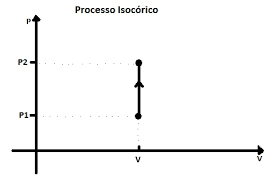
\includegraphics[width=2.5truein]{img9.png}
\caption{Transformação isocórica. Fonte: wikimedia}
\centering
\end{figure}

Aplicando a 1º Lei da Termodinâmica neste tipo de transformação, temos:


\begin{align*}
    \Delta U &= Q - \tau\\
    \Delta U &= Q - 0\\
    \Delta U &= Q
\end{align*}


Isto significa que \textbf{a variação de energia interna sofrida pelo sistema gasoso é igual ao calor trocado com o meio externo}. Sendo assim, temos que considerar duas situações:


\begin{enumerate}

\item{Se sistema recebe calor ($Q>0$), sua energia interna aumenta ($\Delta U>0$) em igual valor.}

\item{Se o sistema cede calor ($Q>0$), sua energia interna diminui em ($\Delta U<0$) em igual valor.}

\end{enumerate}


\hypertarget{x-transformação-isobárica}{\subsection{Transformação Isobárica}}
Nas \textbf{transformações isobáricas, a pressão do sistema gasosos se mantém constante}.


\begin{figure}[h]{}
\centering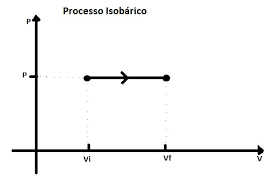
\includegraphics[width=2.5truein]{img10.png}
\caption{Transformação isobárica. Fonte: wikimedia}
\centering
\end{figure}

Dessa forma, a analise do que ocorre é realizada pela de Equação de \textbf{Clapeyron}:


\begin{equation}
    pV=nRT
\end{equation}


Percebemos que, como a pressão é constante, o volume do gás varia em função da temperatura, ou seja, uma variação de volume ($\Delta V$) produz uma variação de temperatura ($\Delta T$). Neste processo de variação de volume, a aplicação da Equação de Clapeyron ficará da seguinte forma:


\begin{equation*}
    p\Delta V=nR\Delta T
\end{equation*}


Nesta transformação, temos que considerar duas situações:


\begin{enumerate}

\item{Quando a temperatura absoluta do sistema aumenta, seu volume também aumenta. Isso significa que sua energia interna aumenta ($\Delta U>0$) e o sistema realiza trabalho ($\tau>0$). Evidentemente, toda a energia entre no sistema na forma de calor.}

\item{Quando a temperatura absoluta do sistema diminui, seu volume também diminui. Isso significa que sua energia interna diminui ($\Delta U<0$) e o sistema recebe trabalho ($\tau<0$). Evidentemente, toda a energia sai do sistema na forma de calor.}

\end{enumerate}


Como estudamos no início, o trabalho realizado por um sistema gasoso a uma pressão constante é dada por:


\begin{equation*}
    \tau = p\Delta V
\end{equation*}


Usando a Equação de Clapeyron:


\begin{equation*}
    \tau = nR\Delta T
\end{equation*}


\hypertarget{x-transformação-adiabática}{\subsection{Transformação Adiabática}}
Nas \textbf{transformações adiabáticas, não há troca de calor entre o sistema e o meio externo}. Portanto, toda a energia recebida ou cedida pelo sistema ocorre por meio do trabalho.


\begin{figure}[h]{}
\centering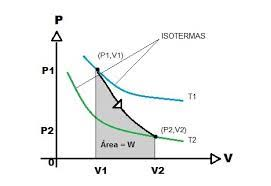
\includegraphics[width=2.5truein]{img11.jpg}
\caption{Transformação adiabática. Fonte: wikimedia}
\centering
\end{figure}

Aplicando a 1º Lei da Termodinâmica neste tipo de transformação, temos:


\begin{align*}
    \Delta U &= Q - \tau\\
    \Delta U &= 0 - \tau\\
    \Delta U &= -\tau
\end{align*}


Isto significa quo o módulo da variação de energia interna sofrida pelo sistema é igual ao módulo do trabalho que o sistema troca com o meio externo. Assim, temos duas situações a considerar:


\begin{enumerate}

\item{Quando o sistema recebe trabalho ($\tau<0$), sua energia interna aumenta ($\Delta U>0$) em igual valor.}

\item{Quando o sistema realiza trabalho ($\tau>0$), ele o faz retirando energia da sua própria energia interna, que diminui ($\Delta U<0$).}

\end{enumerate}


\textbf{Exercício Resolvido 3}


\textbf{(IFG)} As máquinas térmicas são dispositivos que operam sempre em ciclos, isto é, retornam periodicamente às condições iniciais. Uma maneira de estudá-las é por meio de transformações que ocorrem dentro destes ciclos, representados por um gráfico do comportamento da pressão de um gás de trabalho em função do volume por ele ocupado.


O gráfico a seguir representa um ciclo de uma máquina térmica realizado por um sistema gasoso:


\begin{figure}[h]{}
\centering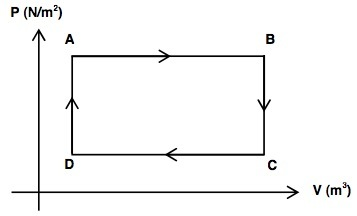
\includegraphics[width=2.5truein]{img16.jpg}
\caption{Diagrama. Fonte: todamateria}
\centering
\end{figure}

Analise as afirmativas.


I - De A para B ocorre uma expansão isobárica. \\
II -  De B para C o trabalho é motor, ou seja, realizado pelo sistema. \\
III - A variação de energia interna no ciclo ABCDA é positiva. \\
IV - No ciclo fechado, ABCDA, não há variação de energia interna e o trabalho total é nulo.


Está(ão) correta(s).


a) Apenas a afirmativa I. \\
b) Apenas as afirmativas I e II. \\
c) Apenas as afirmativas I e IV. \\
d) Apenas as afirmativas I, II e III. \\
e) Apenas as afirmativas I, II e IV.


\begin{resposta*}
{\it I - \textbf{Verdadeiro}. A pressão (representada pelo eixo x) permaneceu constante, caracterizando assim, uma transformação isobárica, enquanto o volume aumentou. \\
II - \textbf{Falso}. Como o volume não varia de B para C, então o trabalho é nula, já que $\tau = p\Delta V$. \\
III - \textbf{Falso}. A variação de energia é nula, pois ao término do ciclo, retorna-se às condições iniciais. \\
IV - \textbf{Falso}. O trabalho realizado não é nulo e pode ser calculado como a área do retângulo formada pelo ciclo. \\
\textbf{Gabarito}: a. $\blacksquare$}
\end{resposta*}

\textbf{Exercício Resolvido 4}


Numa transformação isobárica, $2\;mols$ de um gás perfeito monoatômico recebem uma certa quantidade de calor e consequentemente sua temperatura varia de $300\;K$ a $400\;K$. Determine: \\
a) o trabalho que o gás troca com o meio exterior; \\
b) a correspondente variação de energia interna; \\
c) a quantidade de calor recebida \\
Dado: $R=8,31\;J/(mol\cdot K)$


\begin{resposta*}
{\it a) Primeiramente, vamos calcular o trabalho:
\begin{align*}
    \tau &= p\Delta V \\
    \tau &= nR\Delta T \\
    \tau &= 2\cdot 8,31\cdot (400-300) \\
    \tau &= 1662
\end{align*}

Ou seja, o gás troca com o meio externo um valor de $\boxed{\tau = 1662\;J}$ \\

b) Agora, a variação de energia interna:
\begin{align*}
    \Delta U &= \dfrac{3}{2}nR\Delta T \\
    \Delta U &= \dfrac{3}{2}\cdot 2\cdot 8,31\cdot (400-300)  \\
    \Delta U &= 2493
\end{align*}

Ou seja, nestas condições $\boxed{\Delta U = 2493\;J}$ \\

c) Utilizando a 1° Lei da Termodinâmica
\begin{align*}
    \Delta U &= Q - \tau \\
    Q &= \Delta U + \tau \\
    Q &= 1662 + 2493 \\
    Q &= 4155
\end{align*}

Portanto, $\boxed{Q = 4155\;J}$ $\blacksquare$}
\end{resposta*}

\textbf{Exercício Resolvido 5}


\textbf{(UFLA-MG)} O diagrama $p \times V$ da figura mostra uma transformação sofrida por $0,4\;mol$ de um gás monoatômico ideal.


\begin{figure}[h]{}
\centering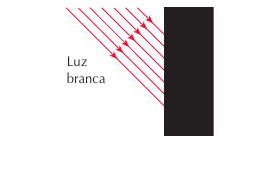
\includegraphics[width=2.5truein]{img12.png}
\caption{Diagrama. Fonte: osfundamentosdafisica}
\centering
\end{figure}

Considerando $T_{A}=300\;K$ e $T_{B}=900\;K$, a quantidade de calor envolvida na transformação será (considere $1\;cal = 4\;J$ e $R = 2\;cal/(mol\cdot K)$):


a) $220\;cal$ \\
b) $-1220\;cal$ \\
c) $2500\;cal$ \\
d) $-2500\;cal$ \\
e) $1220\;cal$


\begin{resposta*}
{\it A área no diagrama $p\times V$ fornece o trabalho. No caso o gás realiza trabalho pois o volume aumenta:
\begin{align*}
    \tau &= \text{Área} \\
    \tau &= (3-1)\times 10^{-3}\cdot 1\times 10^{6} \\
    \tau &= 2\times 10^{3}
\end{align*}

Daí o trabalho realizado é igual a $2\times 10^{3}\;J$ \\

A variação de energia interna é dada por:
\begin{align*}
    \Delta U &= \dfrac{3}{2}nRT \\
    \Delta U &= \dfrac{3}{2}\cdot 0,4\cdot 2\cdot 4\cdot (900-300) \\
    \Delta U &= 2880
\end{align*}

Daí a energia interna é igual a $2880\;J$ \\

Por fim, utilizando a 1ª Lei da Termodinâmica:
\begin{align*}
    \Delta U &= Q - \tau \\
    Q &= \Delta U + \tau \\
    Q &= 2880 + 2000 \\
    Q &= 4880
\end{align*}

Ou seja, o quantidade envolvida nesta transformação foi de $4880\;J$, ou passando para calorias $\boxed{Q=1220\;cal}$ \\
\textbf{Gabarito}: e. $\blacksquare$}
\end{resposta*}

\hypertarget{x-segunda-lei-da-termodinâmica}{\section{Segunda Lei da Termodinâmica}}
Para servir como motivação e estudar os conceitos da \textbf{2ª Lei da termodinâmica}, vamos analisar o seguinte exemplo de um gás sofrendo uma expansão isotérmica $A \Rightarrow B$, como apresentado na figura.


\begin{figure}[h]{}
\centering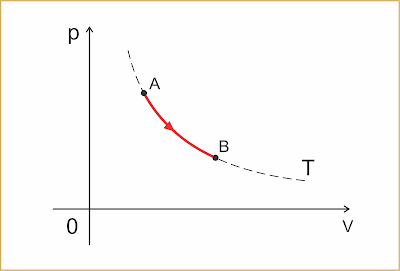
\includegraphics[width=2.5truein]{img13.png}
\caption{Diagrama. Fonte: osfundamentosdafisica}
\centering
\end{figure}

Nesta transformação, a variação de energia interna é nula ($\Delta U=0$).


O gás realiza trabalho ($\tau$) às custas da quantidade de calor ($Q$) recebida. De fato, de acordo com 1ª Lei da Termodinâmica, poder ser sim razoável pensar nesta transformação integral de calor em trabalho, \textbf{mas isso jamais ocorrerá por causas das condições impostas pela 2ª Lei da Termodinâmica}.


\hypertarget{x-máquinas-térmicas}{\subsection{Máquinas Térmicas}}
São denominadas máquinas térmicas os dispositivos usados para converter energia térmica em energia mecânica. Ou seja,
são \textbf{dispositivos que efetuam a conversão de calor em trabalho}.


Esquematicamente:


\begin{figure}[h]{}
\centering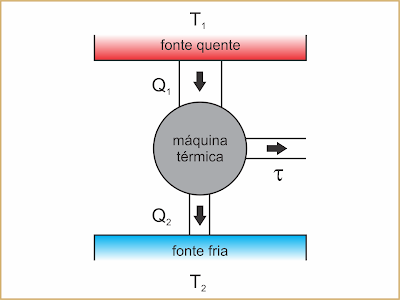
\includegraphics[width=2.5truein]{img14.png}
\caption{Esquema de uma máquina térmica. Fonte: osfundamentosdafisica}
\centering
\end{figure}

O \textbf{rendimento ($\eta$)} de uma máquina térmica, pode ser calculado como a \textbf{razão entre a energia útil obtida em cada ciclo (o trabalho) e a energia total fornecida pela fonte quente (quantidade calor $Q_{1}$)}. Assim:


\begin{equation*}
    \eta = \dfrac{\tau}{|Q_{1}|}
\end{equation*}


O módulo deve-se ao fato de ser apenas computado os valores positivos da quantidade de calor.


Sendo: $\tau = |Q_{1}| - |Q_{2}|$


\begin{align*}
    \eta &= \dfrac{|Q_{1}|-|Q_{2}|}{|Q_{1}|} \\
    \eta &= 1 - \dfrac{|Q_{2}|}{|Q_{1}|}
\end{align*}


Ou seja, o rendimento de uma máquina térmica poder calculado como:


\begin{equation}
    \eta = 1 - \dfrac{|Q_{2}|}{|Q_{1}|}
\end{equation}


É importante ressaltar que, para obter um \textbf{rendimento de $100\%$}, a fonte de calor $Q_{2}$ tem que ser \textbf{nula}, na prática isto é \textbf{impossível}, por causa desta impossibilidade, surgiu o enunciado de \textbf{Kelvin-Planck} para a 2ª Lei da Termodinâmica:


\textbf{É impossível construir uma máquina que, operando em transformações cíclicas, tenha como único efeito transformar completamente em trabalho a energia térmica recebida de uma fonte quente.}


O fato do calor fluir da fonte quente para a fonte fria, levou \textbf{Clausius} a enuncia a 2ª Lei da Termodinâmica da seguinte forma:


\textbf{É impossível uma máquina, sem ajuda de um agente externo, conduzir calor de um sistema para outro que esteja a uma temperatura maior.}


A consequência do enunciado de Clausius é que \textbf{o calor só pode passar de um sistema de menor temperatura para outro de maior temperatura se um agente externo realizar um trabalho sobre esse sistema}, como no caso das \textbf{máquinas frigoríficas}.


Um bom \textbf{refrigerador} (ou condicionador de ar) é aquele que \textbf{retira o máximo de calor da fonte fria ($Q_{2}$) para um mesmo trabalho ($\tau$) realizado pelo motor}. Portanto, quanto mais eficiente for o refrigerador, maior será esta razão. Matematicamente, podemos calcular a eficiência de um refrigerador da seguinte forma:


\begin{equation}
    \eta = \dfrac{Q_{2}}{\tau}
\end{equation}


\hypertarget{x-ciclo-de-carnot}{\subsection{Ciclo de Carnot}}
Até 1824, acreditava-se que uma máquina térmica poderia atingir um rendimento total ($100\%$) ou algo próximo desse valor. Coube ao jovem \textbf{Carnot} demonstrar a impossibilidade desse rendimento.


Ele propôs uma máquina térmica teórica, ideal, que funcionava percorrendo um ciclo particular, denominado \textbf{ciclo de Carnot}. Esse dispositivo obedece a dois postulados, são eles:


\begin{enumerate}

\item{Nenhuma máquina operando entre duas temperaturas fixadas pode ter um rendimento maior que a máquina ideal de Carnot, operando entre essas mesmas temperaturas.}

\item{Ao operar entre duas temperatura, a máquina ideal de Carnot tem o mesmo rendimento, qualquer que seja o fluido operante.}

\end{enumerate}


O ciclo de Carnot é constituído por duas transformações isotérmicas nas temperaturas $T_{1}$ e $T_{2}$, respectivamente das fontes quente e fria, alternadas com duas transformações adiabáticas.


\begin{figure}[h]{}
\centering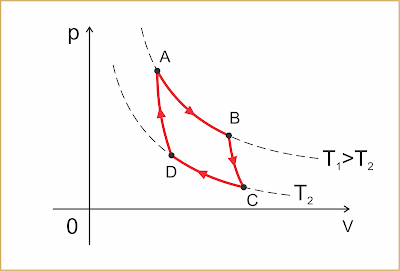
\includegraphics[width=2.5truein]{img15.png}
\caption{Ciclo de Carnot. Fonte: osfundamentosdafisica}
\centering
\end{figure}

\textbf{$A\Rightarrow B$}: expansão isotérmica à temperatura $T_{1}$ (fonte quente). Nesta transformação o gás recebe a quantidade de calor $Q_{1}$.


\textbf{$B\Rightarrow C$}: é a expansão adiabática, na qual a temperatura diminui para $T_{2}$.


\textbf{$C\Rightarrow D$}: compressão isotérmica à temperatura $T_{2}$ (fonte fria). Nesta transformação o gás cede a quantidade de calor $Q_{2}$.


\textbf{$D\Rightarrow A$}: compressão adiabática na qual a temperatura aumenta para $T_{1}$.


O trabalho obtido por ciclo corresponde à área interna dele.


No ciclo de Carnot, vale a seguinte relação:


\begin{equation}
\dfrac{|Q_{2}|}{|Q_{1}|} = \dfrac{T_{2}}{T_{1}}
\end{equation}


Assim, o rendimento de uma máquina térmica operando com o ciclo de Carnot é dado por:


\begin{equation}
\eta = 1- \dfrac{T_{2}}{T_{1}}
\end{equation}


Analisando a relação acima, podemos concluir que:


O \textbf{zero absoluto} seria a temperatura da fonte fria de uma máquina ideal de Carnot, que operasse com rendimento de \textbf{$100\%$}.


\hypertarget{x-entropia}{\subsection{Entropia}}
Em 1865, Clausius introduziu o conceito de \textbf{entropia} para medir a \textbf{desordem de um sistema}. Ele percebeu que se as Leis da Natureza puderem atuar, sem interferências, em um sistema, o mais provável é que os integrantes desse sistema tem a uma disposição desordenada, e o natural é que \textbf{essa desordem do sistema aumente}.


Senso assim, uma nova maneira de enunciarmos a 2ª Lei da termodinâmica seria:


\textbf{Como a entropia é uma medida da desordem e os sistemas físicos tendem para estados cada vez mais desordenados, podemos inferir que, em processos naturais (sujeitos apenas às Leis da Natureza), a entropia do Universo vem aumentando ao longo do tempo}.


Outra informação importante proveniente desta interpretação é que em \textbf{a entropia total de um sistema isolado nunca diminui, somente aumenta ou fica constante}. Acontece que, a entropia somente fica \textbf{constante em processos reversíveis} (aquela em que, após seu término, o sistema pode retornar às suas condições iniciais pelo mesmo caminho), que na realidade são \textbf{ideais}. Na prática, nenhuma transformação é totalmente reversível.


Clausius definiu que a variação de entropia ($\Delta S$) de um sistema, quando se agrega a uma quantidade de calor ($Q$), mediante um processo reversível à temperatura constante ($T$), é dada por:


\begin{equation}
    \Delta S = \dfrac{Q}{T}
\end{equation}


Sendo assim, podemos concluir que:


\begin{enumerate}

\item{Se um sistema recebe calor $Q>0$, sua entropia aumenta ($\Delta S>0$).}

\item{Se um sistema libera calor $Q<0$, sua entropia diminui ($\Delta S<0$).}

\item{Se um sistema não troca calor com o meio externo (transformação adiabática) $Q=0$, a entropia do sistema não varia ($\Delta S=0$).}

\end{enumerate}


Exemplos:


\begin{itemize}

\item \textbf{Copo de vidro quebrando}: o processo de quebra do vidro em pedaços menores é espontâneo, ou seja, é esperado que ocorra quando cai no chão. Dizemos que a entropia, a desordem, desse sistema aumentou. Já o oposto, que o copo volte à altura anterior intacto naturalmente, não é esperado.

\item \textbf{Perfume difundido no ar}: quando abrimos um frasco de perfume, espera-se que o cheiro seja difundido pelo ambiente, pois as moléculas evaporaram no ar, aumentando a entropia do sistema. Não esperamos o oposto, no entanto, que o perfume difundido no ar volte ao frasco quando o abrimos. Ou seja, não seria espontâneo;

\item \textbf{Gelo derretendo}: quando o cubo muda do estado sólido para o líquido sua desordem aumenta, ou seja, aumenta a entropia do sistema. Neste processo, as moléculas se agitam e ficam mais distantes umas das outras, formando um sistema mais desordenado.

\end{itemize}


\textbf{Exercício Resolvido 6}


Considere uma máquina térmica teórica funcionando segundo o ciclo de Carnot entre as temperaturas de $327\;°C$ e $127\;°C$, apresentando um trabalho útil de $800\;J$ por ciclo. Determine, para essa máquina teórica: \\
a) o rendimento. \\
b) a quantidade de calor que, em cada ciclo é retirada da fonte quente. \\
c) a quantidade de calor rejeitada por ciclo para a fonte fria.


\begin{resposta*}
{\it a) Primeiramente, vamos transformar as temperaturas fornecidas na escala Celsius para a escala absoluta Kelvin:

\begin{align*}
T_{1} &= 273+327\\
T_{1} &= 600
\end{align*}

\begin{align*}
T_{2} &= 273+127\\
T_{2} &= 400
\end{align*}

Agora, calculando a rendimento da máquina funcionando segundo o ciclo de Carnot:

\begin{align*}
\eta &= 1-\dfrac{T_{2}}{T_{1}}\\
\eta &= 1-\dfrac{400}{600}\\
\eta &= 1-\dfrac{2}{3}\\
\eta &= \dfrac{1}{3}\\
\eta &= 0,33
\end{align*}

Sendo assim, o rendimento foi de $\boxed{33\%}$ \\

b) Para calcular a quantidade de calor retirada pela fonte quente, vamos utilizar a fórmula do rendimento de uma máquina térmica:

\begin{align*}
\eta &= \dfrac{\tau}{Q_{1}} \\
Q_{1} &= \dfrac{\tau}{\eta} \\
Q_{1} &= \dfrac{800}{\dfrac{1}{3}} \\
Q_{1} &= 800 \cdot 3 \\
Q_{1} &= 2400
\end{align*}

Sendo assim, a quantidade de calor retirada da fonte quente foi de $\boxed{2400\;J}$ \\

c) Por fim, para calcular a quantidade de calor rejeitada para a fonte fria, vamos utilizar o princípio da conservação da energia.

\begin{align*}
Q_{1} &= \tau + Q_{2} \\
Q_{2} &= Q_{1}-\tau \\
Q_{2} &= 2400-800\\
Q_{2} &= 1600
\end{align*}

Sendo assim, a quantidade de calor rejeitada para a fonte fria foi de $\boxed{1600\;J}$ $\blacksquare$}
\end{resposta*}

\textbf{Exercício Resolvido 7}


É possível construir uma máquina térmica, operando entre as temperaturas de $400\;K$ e $300\;K$, que forneça $800\;J$ de trabalho útil, retirando $2000\;J$ da fonte quente?


\begin{resposta*}
{\it O rendimento da máquina seria:

\begin{align*}
    \eta &= \dfrac{\tau}{Q_{1}} \\
    \eta &= \dfrac{800}{2000} \\
    \eta &= 0,40 \\
    \eta &= 40\%
\end{align*}

Agora, o rendimento se a máquina operasse segundo o ciclo de Carnot:

\begin{align*}
    \eta &= 1 - \dfrac{T_{2}}{T_{1}} \\
    \eta &= 1 - \dfrac{300}{400} \\
    \eta &= 1 - \dfrac{3}{4} \\
    \eta &= 0,25 \\
    \eta &= 25\%
\end{align*}

Como sabemos, o \textbf{máximo rendimento teoricamente possível de uma máquina térmica} funcionando entre duas temperaturas $T_{1}$ e $T_{2}$, das fontes quente e fria, é quando opera segundo o \textbf{ciclo de Carnot}. Portanto, podemos concluir que \textbf{não é possível} construir a máquina térmica descrita. $\blacksquare$}
\end{resposta*}

\textbf{Exercício Resolvido 8}


\textbf{(Puc MG)} - Qual dos seguintes estados é o mais desordenado?


a) gás próximo à temperatura de condensação. \\
b) líquido próximo ao ponto de ebulição. \\
c) sólido próximo ao ponto de fusão. \\
d) líquido próximo ao ponto de congelação.


\begin{resposta*}
{\it Em relação aos estados da natureza temos, em geral, o seguinte:

\begin{equation*}
    \Delta S_{\text{gasoso}}>\Delta S_{\text{líquido}}>\Delta S_{\text{sólido}}
\end{equation*}

Ou seja, \textbf{os gases} são mais desordenados do que que um líquido ou um sólido. Portanto, apresentam \textbf{maior entropia}.

\textbf{Gabarito}: a. $\blacksquare$}
\end{resposta*}

\hypertarget{x-exercícios-de-revisão}{\section{Exercícios de Revisão}}
\textbf{1}. Um gás monoatômico e ideal com volume de $3\;m^{2}$ é colocado sobre uma pressão de $10^{6}$ pascal. A energia interna desse gás, em joules, é igual a:


a) $3,0\times 10^{6}\;J$ \\
b) $1,5\times 10^{6}\;J$ \\
c) $5,0\times 10^{6}\;J$ \\
d) $10,0\times 10^{5}\;J$ \\
e) $35\times 10^{5}\;J$


\begin{resposta*}
{\it \textbf{b}}
\end{resposta*}

\textbf{2}. \textbf{(UNIRIO-RJ)} O gráfico mostra uma transformação \textbf{ABC} sofrida por certa massa de gás ideal (ou perfeito), partindo da temperatura inicial $300\;K$.


\begin{figure}[h]{}
\centering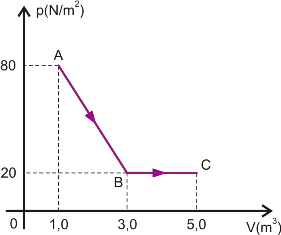
\includegraphics[width=2.5truein]{img17.png}
\caption{Diagrama. Fonte: osfundamentosdafisica}
\centering
\end{figure}

Determine:


a) a temperatura do gás no estado \textbf{C}. \\
b) o trabalho realizado pelo gás na transformação \textbf{AB}.


\begin{resposta*}
{\it a) $275\;K$. \\
b) $100\;J$.}
\end{resposta*}

\textbf{3}. \textbf{(PUC-SP)} O diagrama representa uma transformação cíclica de um gás perfeito.


\begin{figure}[h]{}
\centering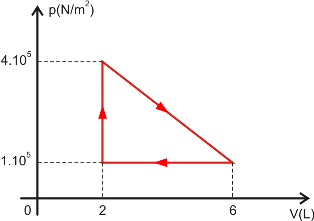
\includegraphics[width=2.5truein]{img18.png}
\caption{Diagrama. Fonte: osfundamentosdafisica}
\centering
\end{figure}

Uma máquina opera segundo este ciclo à taxa de $50$ ciclos por minuto. A potência dessa máquina será igual a:


a) $1\times 10^{4}\;W$ \\
b) $5\times 10^{4}\;W$ \\
c) $1\times 10^{3}\;W$ \\
d) $5\times 10^{5}\;W$ \\
e) $5\times 10^{2}\;W$


\begin{resposta*}
{\it \textbf{e}.}
\end{resposta*}

\textbf{4}. \textbf{(UF Santa Maria-RS)} Um gás ideal sofre uma transformação: absorve $50\;cal$ de energia na forma de calor e expande-se realizando um trabalho de $300\;J$. Considerando $1\;cal = 4,2\;J$, a variação da energia interna do gás é, em J, de:


a) $250$ \\
b) $–250$ \\
c) $510$ \\
d) $–90$ \\
e) $90$


\begin{resposta*}
{\it \textbf{d}}
\end{resposta*}

\textbf{5}. \textbf{(URCA)} Uma máquina térmica utiliza um gás ideal para realizar o ciclo mostrado na figura.


\begin{figure}[h]{}
\centering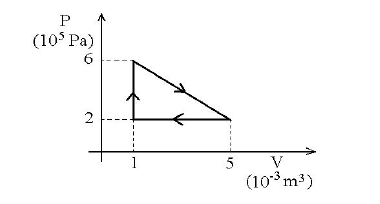
\includegraphics[width=2.5truein]{img19.png}
\caption{Diagrama. Fonte: osfundamentosdafisica}
\centering
\end{figure}

Determine, respectivamente, o trabalho realizado e o calor recebido pelo gás em um ciclo.


a) $1600\;J$ e $–800\;J$. \\
b) $800\;J$ e $1600\;J$. \\
c) $800\;J$ e $800\;J$. \\
d) $1600\;J$ e $–1600\;J$. \\
e) $1500\;J$ e $–1500\;J$.


\begin{resposta*}
{\it \textbf{c}}
\end{resposta*}

\textbf{6}. \textbf{(UECE)} O gráfico abaixo mostra como varia, em função da temperatura absoluta, a energia interna ($U$) de $1\;mol$ de um gás ideal, de massa molar $4\;g/mol$, mantido a volume constante:


\begin{figure}[h]{}
\centering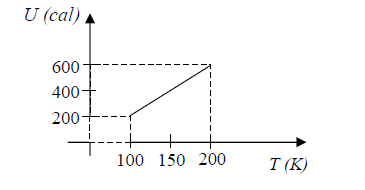
\includegraphics[width=2.5truein]{img20.png}
\caption{Diagrama. Fonte: osfundamentosdafisica}
\centering
\end{figure}

No intervalo mostrado, os valores do trabalho realizado pelo gás nesta transformação, da quantidade de calor que o gás absorveu e do calor especifico (a volume constante), em $cal/(g°C)$ do gás são, respectivamente:


a) $0,\;400,\;4$ \\
b) $0,\;400,\;1$ \\
c) $400,\;0,\;4$ \\
d) $-400,\;400,\;1$


\begin{resposta*}
{\it \textbf{b}}
\end{resposta*}

\textbf{7}. \textbf{(URCA)} O ciclo de Carnot apresenta o máximo rendimento para uma máquina térmica operando entre duas temperaturas. Sobre ele podemos afirmar:


I – É formado por duas transformações adiabáticas alternadas com duas transformações isotérmicas, todas reversíveis; \\
II – A área do ciclo de Carnot é numericamente igual ao trabalho realizado no ciclo; \\
III – As quantidades de calor trocados com as fontes quente e fria são inversamente proporcionais às respectivas temperaturas absolutas das fontes.


Assinale a opção que indica o(s) item(ns) correto(s):


a) I, II e III. \\
b) Somente I e III. \\
c) Somente II e III. \\
d) Somente I. \\
e) Somente I e II.


\begin{resposta*}
{\it \textbf{e}}
\end{resposta*}

\textbf{8}. Uma máquina térmica recebe da fonte quente, em cada ciclo, uma quantidade de calor de $2000\;J$. Sabendo-se que o rendimento da máquina é de $10\%$, determine:


a) o trabalho que a máquina realiza em cada ciclo. \\
b) a quantidade de calor rejeitada para a fonte fria.


\begin{resposta*}
{\it a) $200\;J$. \\
b) $1800\;J$.}
\end{resposta*}

\textbf{9}. \textbf{(UFLA-MG)} Uma empresa propõe construir um motor térmico projetado para operar entre dois reservatórios de calor, sendo o quente à temperatura $T_{1} = 1600\;K$ e o frio a $T_{2} = 400\;K$. O projeto prevê, para o motor, uma potência de $4\;cv$, com absorção de $1480\;cal/s$ do reservatório quente. \\
Dados: \\
$1\;cv = 740\;W$. \\
$1\;cal = 4\;J$.


a) Calcule o rendimento do referido motor. \\
b) Calcule o rendimento de um motor de Carnot, operando entre os mesmos reservatórios de calor. \\
c) O motor proposto é viável teoricamente? Justifique sua resposta.


\begin{resposta*}
{\it a) $50\%$. \\
b) $75\%$. \\
c) Sim, é viável.}
\end{resposta*}

\textbf{10}. \textbf{(UFOP MG/2008)} Com relação à entropia e à segunda lei da termodinâmica, é incorreto afirmar:


a)	Ciclo termodinâmico é um processo em que uma máquina térmica ou um sistema termodinâmico volta a seu estado inicial. \\
b)	Não existe máquina térmica que transforme todo calor de uma fonte em trabalho. \\
c)	A diluição de uma gota de tinta em um copo de água é um exemplo de processo reversível. \\
d)	Em todo processo isolado irreversível, a entropia total do sistema sempre aumenta.


\begin{resposta*}
{\it \textbf{c}}
\end{resposta*}

\hypertarget{x-referências}{\section{Referências}}
CALÇADA, Caio Sérgio; SAMPAIO, José Luiz. Física Clássica: Termologia, Óptica e Ondas. Atual Editora, São Paulo, 2012.


CAMPOS, Bruna Manuele. "Entropia – O que é? Características, Fórmula, Exemplos e Exercícios". Gestão Educacional. Disponível em: \href{https://www.gestaoeducacional.com.br/entropia-o-que-e-caracteristicas/}{https://www.gestaoeducacional.com.br/entropia-o-que-e-caracteristicas/}


FERRARO, Nicolau Gilbert. "Termodinâmica". Blog Os Fundamentos da Física. Disponível em: \href{https://osfundamentosdafisica.blogspot.com/}{https://osfundamentosdafisica.blogspot.com/}


RAMALHO JR, Francisco; FERRARO, Nicolau Gilberto; SOARES, Paulo Antônio de Toledo. Os Fundamentos da Física vol. 2. \textbf{Moderna, São Paulo}, 2007.


VILLAS BÔAS, Newton; DOCA, Ricardo Helou; BISCUOLA, Gualter José. Tópicos de física, 2: termologia, ondulatória e óptica. \textbf{São Paulo: Saraiva}, 2012.


\end{document}

